\documentclass[11pt]{article}

\usepackage[margin=1in]{geometry}
\usepackage{graphicx}
\usepackage{booktabs}
\usepackage{amsmath}
\usepackage{amssymb}
\usepackage{hyperref}
\usepackage{xcolor}
\usepackage{tikz}
\usetikzlibrary{arrows.meta, positioning, calc, fit}

\title{\textbf{zklora: Verifiable Multi-Party Inference for Evaluating Private LoRA Weights}}
\author{Anonymous Authors}
\date{\today}

\begin{document}

\maketitle

\begin{abstract}
In decentralized computing environments, one party may wish to fine-tune a publicly available base model with Low-Rank Adaptation (LoRA) but keep those adapter weights private, while another party wants to evaluate performance on new data. 
We introduce \texttt{zklora}, a library designed to help the \emph{Base Model User} \emph{verifiably assess} the quality of a private LoRA module for a target task---for instance, to run a validation experiment without directly accessing the private weights. 
By adopting a multi-party inference approach and generating \emph{verifiable computations}, \texttt{zklora} enables the \emph{Base Model User} to confirm that remote LoRA computations are correct, all without seeing the private weights themselves. 
We demonstrate the feasibility of \texttt{zklora} via benchmark experiments, showing that our approach remains computationally viable across various model sizes, with notably fast verification times.
\end{abstract}

%------------------------------------------
% Move INTRO to the beginning
%------------------------------------------
\section{Introduction}
Large Language Models (LLMs) excel at many tasks but can be expensive to store and fine-tune \cite{brown2020language, devlin2018bert}. 
Low-Rank Adaptation (LoRA) \cite{hu2021lora} addresses these costs by injecting small adapter matrices, making specialized fine-tuning more efficient \cite{ding2022delta}. 

However, if a \emph{LoRA Owner} wants to keep these weights private while a \emph{Base Model User} needs to validate them on a local dataset, a direct sharing of the LoRA parameters is impossible. \texttt{zklora} solves this dilemma by orchestrating multi-party inference: The Base Model User runs the base model layers locally, forwarding partial activations to the LoRA Owner for the private transform. A zero-knowledge proof is generated to demonstrate correctness, ensuring that final performance metrics are truly representative of the private LoRA.

%------------------------------------------
% 1. PRELIMINARY RESULTS
%------------------------------------------
\section{Preliminary Results}

We benchmarked \texttt{zklora} by measuring the creation and verification times across multiple base models and private LoRA configurations. 
Figures~\ref{fig:settings}, \ref{fig:proof}, and \ref{fig:verify} show the total LoRA parameter count (horizontal axis) versus:
\begin{itemize}
    \item \textbf{Total Settings Time} (sec),
    \item \textbf{Total Proof Generation Time} (sec),
    \item \textbf{Total Verification Time} (sec),
\end{itemize}
respectively.

\begin{figure}[ht]
    \centering
    \includegraphics[width=0.55\linewidth]{figs/fig_settings.pdf}
    \caption{Total LoRA params (in millions) vs. total settings time. Each point is a different model.}
    \label{fig:settings}
\end{figure}

\begin{figure}[ht]
    \centering
    \includegraphics[width=0.55\linewidth]{figs/fig_proof.pdf}
    \caption{Total LoRA params (in millions) vs. total proof generation time. Each point is a different model.}
    \label{fig:proof}
\end{figure}

\begin{figure}[ht]
    \centering
    \includegraphics[width=0.55\linewidth]{figs/fig_verify.pdf}
    \caption{Total LoRA params (in millions) vs. total verification time. Each point is a different model.}
    \label{fig:verify}
\end{figure}

Notably, while proof-generation times can grow with model size, verification remains consistently fast (on the order of 1--2 seconds per proof for large models). This helps real-world “trial runs,” letting the Base Model User confirm private LoRA quality without incurring excessive overhead.

%------------------------------------------
% 2. MULTI-PARTY INFERENCE METHOD
%------------------------------------------
\section{Multi-Party Inference: zklora for Verifiable Evaluation}

Our approach allows the \emph{Base Model User} to incorporate a private LoRA module from the \emph{LoRA Owner}:

\begin{enumerate}
    \item \textbf{Base Model Forward Pass.} 
    The user runs all layers without LoRA locally, producing partial activations.

    \item \textbf{Forward to LoRA Adapter.} 
    The partial activations are sent to the LoRA Owner for private transformations.

    \item \textbf{LoRA Computation \& Proof Generation.} 
    The LoRA Owner updates the activations and produces a zero-knowledge proof of correctness.

    \item \textbf{Resuming the Forward Pass.} 
    The updated activations are returned and merged into the local forward pass.

    \item \textbf{Verification \& Validation.} 
    The Base Model User verifies the proof and measures final metrics (e.g., accuracy) to decide if the LoRA meets their needs.
\end{enumerate}

\begin{figure}[ht]
\centering
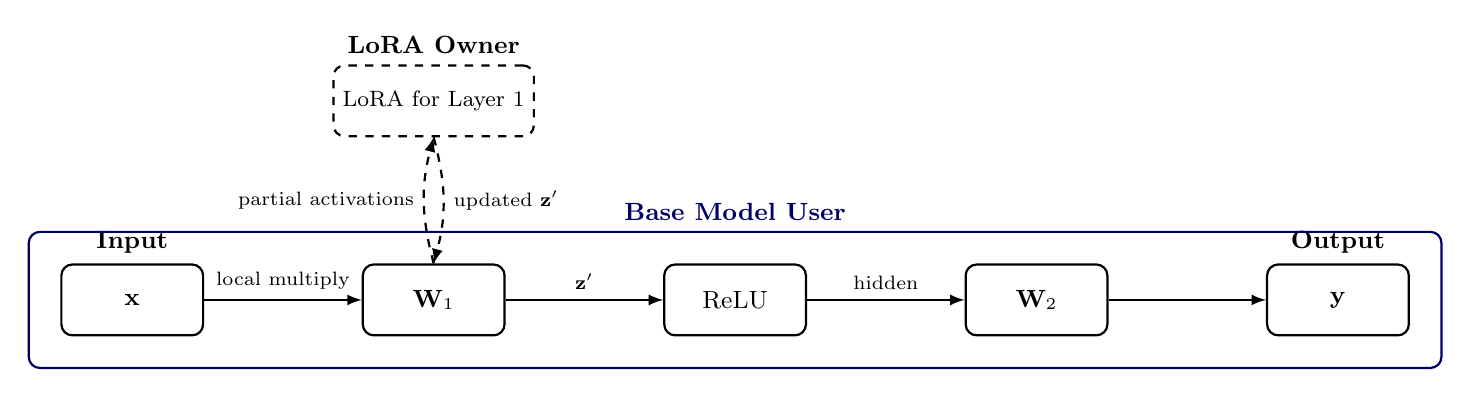
\begin{tikzpicture}[
    font=\small,
    >=latex,
    thick,
    block/.style={
      draw,
      rounded corners,
      align=center,
      minimum width=1.8cm,
      minimum height=0.9cm
    },
    dashedblock/.style={
      draw,
      dashed,
      rounded corners,
      align=center,
      font=\footnotesize,
      fill=white,
      minimum width=1.8cm,
      minimum height=0.9cm
    },
    arrow/.style={->, thick},
    node distance=2.0cm
]

\node[block, label=above:\textbf{Input}] (input) {$\mathbf{x}$};
\node[block, right=2.0cm of input] (W1) {$\mathbf{W}_1$};
\node[dashedblock, above=1.6cm of W1, label=above:\textbf{LoRA Owner}] (LoRA) {LoRA for Layer 1};
\node[block, right=2.0cm of W1] (act) {ReLU};
\node[block, right=2.0cm of act] (W2) {$\mathbf{W}_2$};
\node[block, label=above:\textbf{Output}, right=2.0cm of W2] (output) {$\mathbf{y}$};

\draw[->] (input) -- node[above, font=\scriptsize]{local multiply} (W1);
\draw[->, dashed] (W1.north) to[bend left=15] node[left, font=\scriptsize]{partial activations} (LoRA.south);
\draw[->, dashed] (LoRA.south) to[bend left=15] node[right, font=\scriptsize]{updated $\mathbf{z}'$} (W1.north);
\draw[->] (W1) -- node[above, font=\scriptsize]{$\mathbf{z}'$} (act);
\draw[->] (act) -- node[above, font=\scriptsize]{hidden} (W2);
\draw[->] (W2) -- (output);

\node[draw, rounded corners, thick, color=blue!40!black,
      fit=(input)(W1)(act)(W2)(output),
      label={[font=\small, color=blue!40!black]above:\textbf{Base Model User}},
      inner sep=0.4cm
] (baseModelFit) {};
\end{tikzpicture}
\caption{A simplified 2-layer MLP with LoRA on the first layer. The Base Model User (blue box) runs most computations locally, then requests the LoRA Owner (dashed box) to update partial activations.}
\label{fig:toy-mlp-lora}
\end{figure}

%------------------------------------------
% 3. HOW WE GENERATE THE ZERO-KNOWLEDGE PROOF
%------------------------------------------
\section{Generating the Zero-Knowledge Proof}

Central to \texttt{zklora} is the cryptographic proof that the LoRA computations were conducted faithfully. Below is a high-level outline:

\paragraph{Circuit Compilation (Model + JSON Input).}
The LoRA Owner provides an ONNX model that includes the LoRA parameters. We compile it into a “circuit” representing the layer computations. Next, the Base Model User's partial activations, saved as JSON, feed into this circuit as inputs.

\paragraph{Settings and Key Generation.}
We produce (1) a “settings” file that includes circuit metadata, (2) a proving key (PK) and verification key (VK), and optionally (3) a structured reference string (SRS) for polynomial commitments.

\paragraph{Witness Creation.}
We run the partial activations through the circuit, storing all intermediate wire values in a “witness” file that reflects the correct usage of the LoRA layer.

\paragraph{Proving.}
Using the PK, the witness, and the circuit, the LoRA Owner generates a proof file. This file certifies that the LoRA transformation was done correctly, matching the declared ONNX logic.

\paragraph{Verification.}
The Base Model User loads the proof and verifies it with the VK (plus SRS). If it checks out, the user trusts that the LoRA updates are accurate, without ever seeing the LoRA weights directly.

%------------------------------------------
% 4. RELATED WORK
%------------------------------------------
\section{Related Work}

\subsection{Low-Rank Adaptation}
LoRA \cite{hu2021lora} is widely adopted for parameter-efficient fine-tuning across GPT-2, GPT-Neo, and LLaMA. By focusing updates on low-rank adapters, it reduces memory overhead \cite{ding2022delta}.

\subsection{Incrementally Verifiable Computation}
Earlier cryptographic frameworks \cite{valiant2008incrementally, kothapalli2022nova, kothapalli2024hypernova} show how to prove correctness of multi-step computations. \texttt{zklora} combines these proof techniques with a multi-party inference flow, ensuring that LoRA transformations remain private yet verifiable.

%------------------------------------------
% 5. CONCLUSION
%------------------------------------------
\section{Conclusion}

We present \texttt{zklora} as a verifiable multi-party inference solution to validate private LoRA adapters. Our benchmarks show that proof generation scales with model size, while verification remains consistently quick. This enables the Base Model User to run iterative experiments on LoRA modules without risking the LoRA Owner’s privacy. Future extensions might explore multi-owner LoRA composition or advanced multi-party computation frameworks that guard both user data and model parameters with cryptographic guarantees.

\bibliographystyle{plain}
\bibliography{references}

\end{document}
